% Einstellen der Dokumentenklasse (möglich: book, report, article, dinbrief, beamer, scrbook, scrreprt, scrartcl)
% Einstellen der Dokumentoptionen (möglich: 11pt, twocolumn, oneside, titlepage, landscape, a4paper)
\documentclass[12pt,a4paper]{report}

% Template einbinden. Mögliche optionen:
%		chapter, section: 							definiert die oberste Gliederungsebene (default = chapter)
% 	header-line, no-header-line: 		Ein- bzw. Ausschalten der Kopfzeilentrennlinie (default = header-line)
% 	footer-line, no-footer-line: 		Ein- bzw. Ausschalten der Fußzeilentrennlinie (default = footer-line)
% 	switchhf: 											tauschen der Kopf- und Fußzeile
% 	last-page: 											Ein- bzw. Ausschalten der Gesamtseitenanzeige
% 	block:													Blocksatzformatierung aktivieren
\usepackage[onehalfspacing]{setspace}
\usepackage[]{template}

\usepackage{listings}
\usepackage{color}
\usepackage{acronym}
\usepackage{svg}

\definecolor{dkgreen}{rgb}{0,0.6,0}
\definecolor{gray}{rgb}{0.5,0.5,0.5}
\definecolor{mauve}{rgb}{0.58,0,0.82}

\lstset{frame=tb,
	language=Java,
	aboveskip=3mm,
	belowskip=3mm,
	showstringspaces=false,
	columns=flexible,
  basicstyle={\small\ttfamily},
  numbers=left,
  numberstyle=\tiny\color{gray},
  keywordstyle=\color{blue},
	commentstyle=\color{dkgreen},
	stringstyle=\color{mauve},
	breaklines=true,
	breakatwhitespace=true,
  tabsize=3,
  captionpos=b 
}
\usepackage{enumitem}
\setlist[description]{style=nextline}

\newcommand*{\captionsource}[1]{%
      \textbf{Quelle:} #1%
  }%

% Dokumentinformationen einbinden
% Meta-Tags
\hypersetup{
	colorlinks,
	linkcolor={black},
	citecolor={black},
	urlcolor={black},
	pdftitle={},
	pdfsubject={},
	pdfauthor={},
	pdfkeywords={},
	pdfcreator={latexmk}
}

% Dokumentinformationen
\author{Frederick Lahde, Lars Grahmann}
\title{Chromstahl-CMS}
\date{\today}

% Informationen für die Kopf- und Fußzeile
\renewcommand{\subject}{Chromstahl-CMS}
\renewcommand{\topic}{}

\begin{document}
	% Titelseite
	\maketitlenew

	% Inhaltsverzeichnis
	\tableofcontentsnew
	\newpage

	% Start here
  \listoffigures
  \clearpage
  \textbf{Genderhinweis}\\
Aus Gründen der Lesbarkeit wurde im Text die männliche Form gewählt, nichtsdestoweniger beziehen sich die Angaben auf Angehörige beider Geschlechter.
  \chapter{Abkürzungsverzeichnis}
\begin{acronym}[Virtual DOM]
  \acro{DOM}{Document Object Model}
  \acro{VDOM}[Virtual DOM]{Virtual Document Object Model}
  \acro{REST}{Representational State Transfer}
  \acro{MVVM}{Model-View-ViewModel}
  \acro{CMS}{Content-Management-System}
  \acro{CaaS}{Content as a Service}
  \acro{RBAC}{Rolebased Access Control}
  \acro{SDK}{Software Development Kit}
  \acro{CMA}{Content Management Application}
  \acro{CDA}{Content Delivery Application}
  \acro{DBMS}{Database Management System}
  \acro{ERM}{Entity Relationship Model}
  \acro{SPA}{Single Page Application}
  \acro{XML}{Extensible Markup Language}
  \acro{API}{Application Programming Interface}
  \acro{HTML}{Hypertext Markup Language}
\end{acronym}

  \chapter{Einleitung}
Das Thema der Projektarbeit ist die umsetzung einer modernen \ac{CMS} Lösung. Hierbei wurde besonders auf eine von grund auf modulare Architektur geachtet. Diese ist umgesetzt mithilfe des \ac{MVVM} Entwurfsmusters. Ziel dabei ist es, eine stabile und leicht zu erweiternde Basis für eine Vielzahl von Implementationen für Webanwendungen zu schaffen.

\section{Motivation}
% TODO: Maybe add some studies here?
Mehr denn je ist es in der Softwareentwicklung erforderlich, schnell und zuverlässig auf Kundenwünsche reagieren zu können. \acs{CMS} Lösungen schaffen eine solide Grundlage, die erprobte Lösungen für immer wiederkehrende Proleme, wie beispielsweise Authentifikation und Gruppenmanagement bereitstellen.

\section{Aufbau der Arbeit}
\begin{description}
\item[Kapitel 1:]{Das erste (dieses) Kapitel behandelt das Thema und die Motivation der Projektarbeit. Desweiteren wird der Aufbau der Arbeit erläutert}
\item[Kapitel 2:]{In der theoretischen Betrachtung werden grundlegende Konzepte eingeführt. Der Leser entwickelt Hintergrundwissen, welches insbesonders in der Umsetzung benötigt werden.}
\item[Kapitel 3:]{Unter dem Sitchwort Methodik werden Technologieentscheidungen erörtert, die im Laufe des Projektes getroffen wurden. Für verschiedene Probleme werden Lösungen diskutiert und eine Entscheidung begründet.}
\item[Kapitel 4:]{Die Umsetzung behandelt die tatsächliche Implementation des Projektes. Wichtige Datenstrukturen und Spezifikationen werden erläutert und diverse Code-Listings geben einen umfassenden Überblick über die Realisierung.}
\item[Kapitel 5:]{Im fünften Kapitel werden anfängliche Entscheidungen und Betrachtungen retrospektivischaufgegriffen und in Hinsicht auf die Erfahrungen im Projekt diskutiert}
\item[Kapitel 6:]{Am Ende der Arbeit steht eine Zusammenfassung. Es wird auf die tatsächlich Umsetzung der Ziele eingegangen und ein Ausblick gegeben.}
\end{description}

  \chapter{Theoretische Betrachtung}
\section{\acl{CMS}}
\subsection{\acl{CMA}}
\subsection{\acl{CDA}}
\subsection{Bestehende Lösungen}
\subsubsection{Wordpress}
\subsubsection{Joomla}
\subsubsection{Drupal}

\section{\acl{DOM}}
\subsection{Standards}
\ac{XML} bildet eine Dokumenthierarchie ab, welche einen maschinell lesbaren Aufbau eines
Dokumentes, mithilfe von einer generischen Syntax, definiert. \ac{XML} wird in
verschiedenen Formen in vielen Geräten und Programmen genutzt um Datenstrukturen
abzubilden. Diese Datenstrukturen können in verschiedenen, Domäne-spezifischen
varianten beschrieben werden, wie zum Beispiel

\begin{itemize}
\item Scalable Vector Graphic (SVG)
\item Rich Site Summary (RSS)
\item Extensible Hypertext Markup Language (XHTML)
\end{itemize}

Das \ac{DOM} definiert ein \ac{API} zum manipulieren von \ac{XML} als
Baumstruktur. \cite{harold}

\subsection{Aufbau}
\begin{figure}
  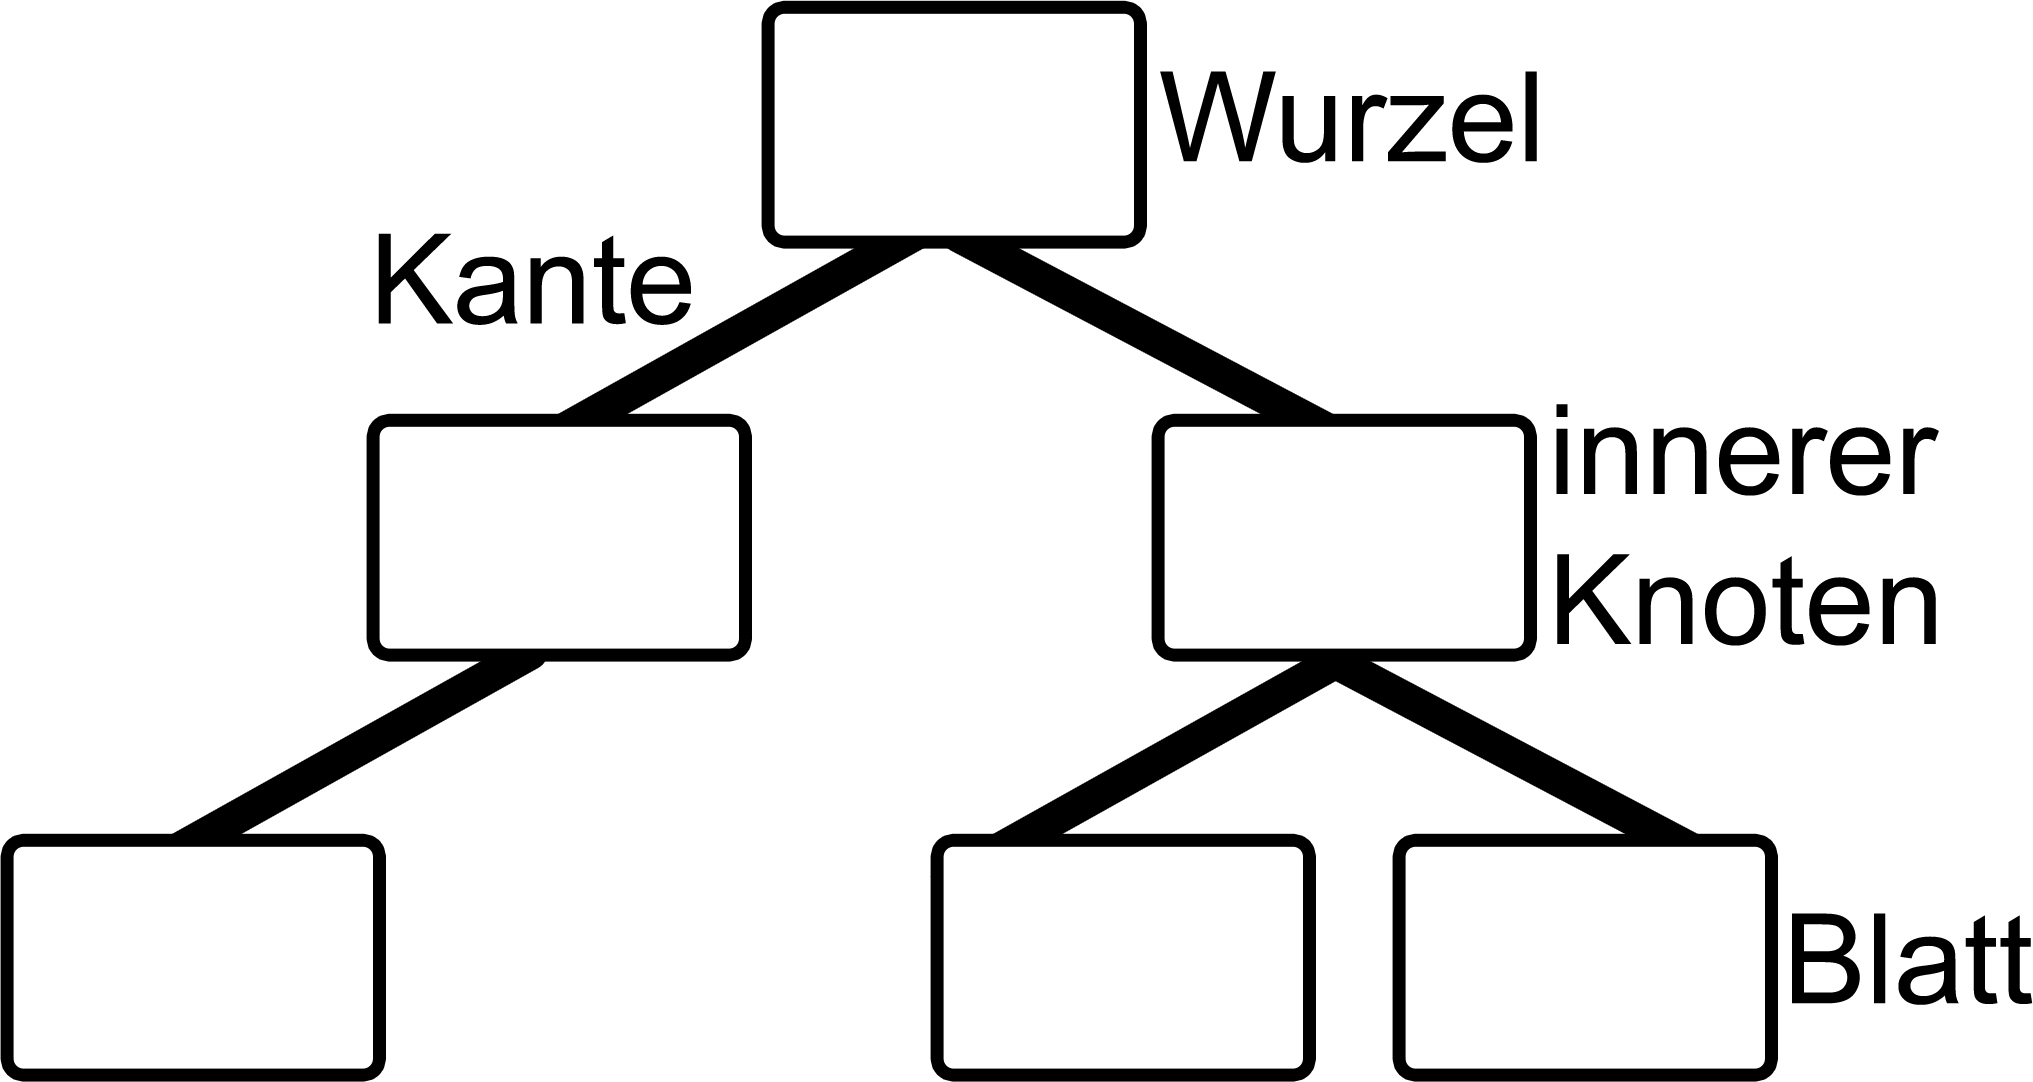
\includegraphics[width=\linewidth]{images/binarytree.jpg}
  \caption{Baumstruktur}
  \captionsource{Von Mhombach - Eigenes Werk, CC BY-SA 3.0, https://commons.wikimedia.org/w/index.php?curid=29981537}
  \label{fig:binarytree}
\end{figure}

Eine Baumstruktur (\ref{fig:binarytree}) besteht aus einem Wurzel-knoten,
welcher mithilfe von Kanten ``Kind knoten'' oder auch ``innere Knoten'' besitzen
kann. Hat ein Knoten keine ``Kinder'', wird er als ``Blatt'' bezeichnet.
Baumstrukturen sind für die Darstellung von Daten aufgrund ihrer einfachen
Gestaltung vorteilhaft. Eine Baumstruktur kann sehr leicht mithilfe von
rekursiven Funktionen durchlaufen werden, da ein Knoten immer genau ein
``Elternteil'' und eine Liste von ``Kindern'' hat.

\section{\acl{VDOM}}
\subsection{Definition}

Ein \ac{VDOM} ist eine Repräsentation eines \ac{DOM} welche durch arbiträre
Datenstrukturen abgebildet werden kann. Eine häufige Implementation ist durch
Javascript-Objekte, welche die Daten des \ac{DOM} abbilden.

\subsection{Motivation}

Oft wird ein \ac{VDOM} verwendet, da aus manipulation der Daten automatisch eine
Änderung im \ac{DOM} abgebildet werden kann, und somit der Entwickler lediglich
die Änderung der Daten bedenken muss.

\subsection{Nachteile}

Eine Repräsentation des \ac{DOM} als \ac{VDOM} führt zwangsläufig dazu, dass die
Struktur des \ac{DOM} doppelt vorhanden ist. Desweiteren ist das finden der
Änderungen zwischen \ac{DOM} und \ac{VDOM} nicht trivial und langsamer als eine
``direkte'' Änderung der Daten im \ac{DOM}. Weiterhin muss der Web-Browser
zusätzlich zum finden der Änderungen zwischen \ac{DOM} und \ac{VDOM} immer
die \ac{DOM}-\ac{API} Aufrufe ausführen.

\section{\acl{SPA}}
Eine \ac{SPA} beschreibt eine Web-Applikation, die auf einer Webseite abgebildet ist. Dies wird realisiert, indem die gesamte Präsentationslogik, im Kontrast zu traditionellen Webanwendungen, im Browser implementiert wird.\cite{SPA} 
\subsection{Unterscheidung}
\subsubsection{Traditionelle Webanwendung}
\begin{figure}
  \begin{center}
    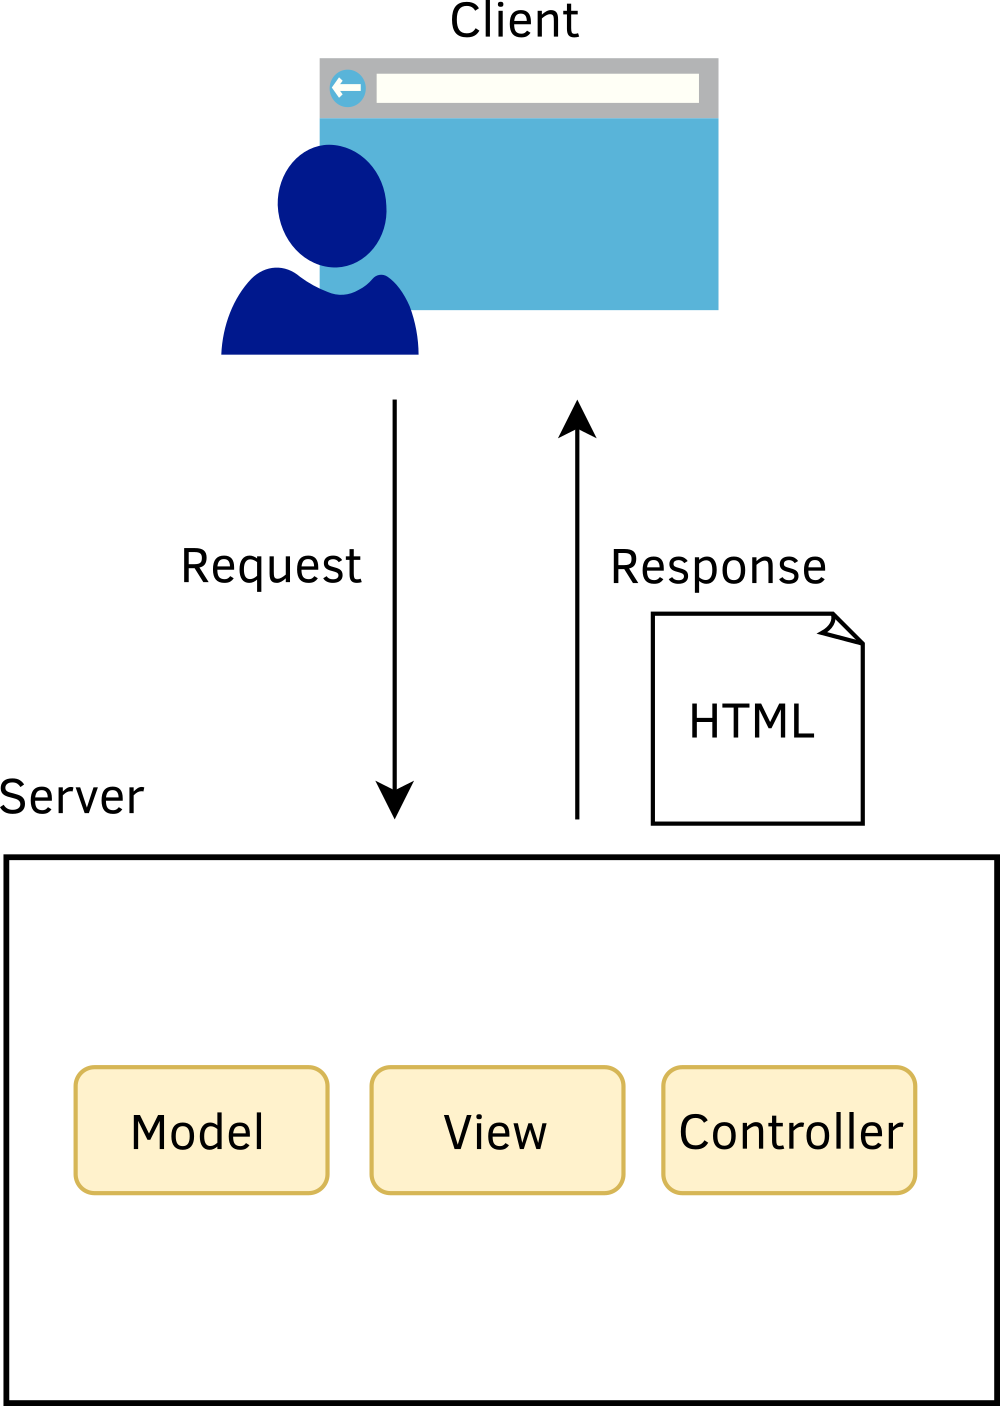
\includegraphics[scale=1]{images/traditonal_web_app.png}
  \end{center}
  \caption{Traditionelle Web Anwendung}
  \captionsource{Eigenes Werk}
  \label{fig:tradweb}
\end{figure}
Traditionelle Webanwendungen (siehe Abbildung \ref{fig:tradweb}) lösen bei jeder Anfrage des Nutzers einen Roundtrip \footnote{Senden einer Anfrage an einen Server und Erhalt der entsprechenden Antwort} aus zum Server aus.\\
Server-seitig wird der Request von einem Controller entgegengenommen. Dieser agiert mit dem Model, welches die benötigten Daten liefert (beispielsweise durch eine Anfrage an eine Datenbank). Die Logik im Controller bestimmt anschließend das benötigte View und füllt dieses mit Daten.\\
Der Server antwortet mit einem \ac{HTML} Dokument und der Browser stellt dies nach einer Aktualisierung der gesamten Webseite dar.
\subsubsection{\acl{SPA}}
\begin{figure}
  \begin{center}
    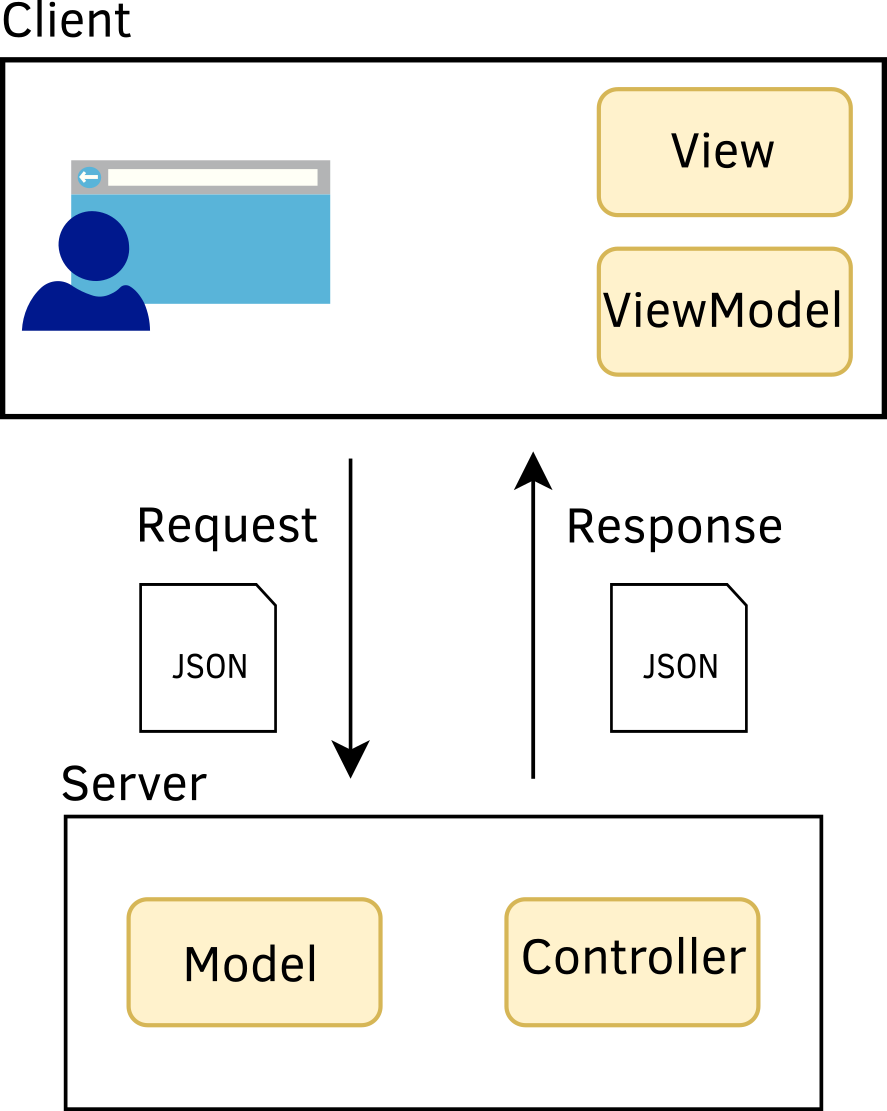
\includegraphics[scale=1.5]{images/spa_web_app.png}
  \end{center}
  \caption{\acl{SPA}}
  \captionsource{Eigenes Werk}
  \label{fig:spaweb}
\end{figure}
Bei einer \ac{SPA} hingegen wird die gesamte View Logik in den Client verlagert
(siehe Abbildung \ref{fig:spaweb}). Die Kommunikation mit dem Server reduziert
sich bei dieser Architektur auf reinen Austausch von Daten.\\
Eine Aktion des Nutzers, beispielsweise ein Klick auf einen Button, wird behandelt indem das
View die Aktion an das Viewmodel weiterleitet. Das Viewmodel aktualisiert den
lokalen Zustand (State) der Anwendungen und stell bei Bedarf eine Anfrage an den Server um Daten auszutauschen und aktualisiert anschließend
das View.\\
Dies hat diverse Auswirkungen auf die Anwendung: 
\begin{description}
  \item[Keine Aktualisierungen der gesamten Seite]In einer \ac{SPA} werden Views
    nicht als gesamte \ac{HTML} Seite abgebildet. Vielmehr ist ein View als ein
    Teil des \ac{DOM} anzusehen, welches zum richtigen Zeitpunkt mit dem
    vorhergegangen View ausgetauscht wird. Nach dem initialen Laden der Seite
    gibt es keine weiteren Aktualisierungen dieser.\\
    Aus Sicht der \ac{UX}
    gleicht dies mehr einer nativen Smartphone App als einer Webseite. Dies
    führt zu einer vertrauteren Umgebung, insbesondere wenn die Anwendung auf
    einem Smartphone oder Tablet benutzt wird.
  \item[Trennung von Client und Server]Durch die Verlagerung der
    View Logik wird eine klare Abgrenzung zwischen Client und Server erreicht.
    Die Kommunikation wird durch eine \ac{REST} Spezifikation ausgedrückt und
    somit ist sowohl der Client als auch der Server leicht austuschbar. Diese
    Entkopplung ist bekannt unter dem Ausdruck ``single responsibility principle''\cite{cleancode}.
\end{description}

\section{Datenstrukturen}
\subsection{\acl{DBMS}}
\subsection{\acl{ERM}}
\section{Plug-in}
Modularität war von Anfang an ein wichtiger Gesichtspunkt bei der Entwicklung
von Chromstahl. Es sollte möglich sein, das \ac{CMS} effizient an neue Aufgaben
anzupassen, beispielsweise für ein Video Portal. Eine solche Modularität lässt
sich über Plug-ins realisieren.
\subsection{Definition}
Ein Plug-in (auch Add-on genannt) ist eine Komponente die eine spezielle
Funktion zu einer bestehenden Software
hinzufügt.\footnote{https://en.wikipedia.org/wiki/Plug-in\_(computing)}
\subsection{Implementationsansätze}
% TODO: flesh this out
Zu Beginn des Projektes wurden zwei Ansätze zur Implementierung von Plug-ins für
Chromstahl konzipiert. Diese werden im folgenden erläutert und im späteren
Verlauft dieser Arbeit konkret behandelt.
\subsubsection{Dynamisch}
Der erste Ansatz war das dynamische Laden von Plug-ins. Dies bedeutet, dass
Plug-ins zur Laufzeit aufgelöst und geladen werden. 
\subsubsection{Statisch}
% LocalWords:  Superset

  \chapter{Methodik}
\section{Vergleich von Web-Frontend Sprachen}
Es gibt eine Vielzahl von möglichen Programmiersprachen zur Erstellung von
Web-Frontends. Zu Beginn des Projektes wurden daher verschiedene Sprachen
evaluiert. Nachfolgend die Ergebnisse unserer Betrachtungen.
\subsection{Javascript}
Nach dem ersten Erscheinen am 4. Dezember
1995\footnote{https://web.archive.org/web/20070916144913/http://wp.netscape.com/newsref/pr/newsrelease67.html}
entwickelte sich \ac{JS} neben \ac{HTML} und \ac{CSS} schnell zu einer der Kern
Technologien des Web.\\
Die Syntax von \ac{JS} basiert, genau wie etwa C oder
Java, auf geschweiften Klammern. Es werden diverse Paradigma wie Funktionale und
Objekt Orientierte Programmierung unterstützt. \acl{JS} liefert eine umfangreiche
Standardbibliothek mit einer einer Vielzahl von
\ac{API}s zum Manipulieren eines \ac{DOM}s. Die Sprache ist
dynamisch\footnote{https://en.wikipedia.org/wiki/Type\_system\#Combining\_static\_and\_dynamic\_type\_checking}
typisiert.
\subsection{\acl{TS}}
\ac{TS} ist ein von Microsoft entwickeltes Superset von
\acl{JS}\footnote{https://www.typescriptlang.org}. Es erweitert \ac{JS} um eine
optional verwendbare strikte Typisierung, die beim Übersetzen zu \ac{JS}
überprüft wird. Dies hat zwei Vorteile gegenüber einer dynamischen Sprache wie
beispielsweise \acl{JS}\footnote{https://pchiusano.github.io/2016-09-15/static-vs-dynamic.html}:
\begin{description}
  \item[Entdecken von Fehlern zur Kompilierzeit]{Viele semantische Fehler werden
    während des Kompilierens erkannt. Hierzu gehören Fehler wie das Übergeben
    von Parametern eines falschen Typs in eine Funktion oder das aufrufen einer
    Funktion, die nicht existiert}
  \item[Bessere Lesbarkeit]{Statisch typisierter Quellcode ist für den
      Programmierer einfacher lesbar, da Typen von Parametern und Variablen
      direkt ersichtlich sind und nichts aus dem Name oder dem Kontext
      herausgefunden werden müssen}
  \item[Bessere Editor Untersützung]{Dadurch, dass Typinformationen zur
      Kompilierzeit zur Verfügung stehen, kann der Editor dem Programmierer eine
      bessere Autovervollständigung bieten}
\end{description}
Ein Nachteil von \acl{TS} ist die Tatsache, dass Typinformationen von externen
Softwarebibliotheken für die vollständige Überprüfung des Typsystems
vorhanden sein müssen. Ein Großteil von \ac{JS} Bibliotheken wird ohne diese
Informationen geliefert, weshalb für diese Typinformationen von der Community
verwendet werden, die nicht zwingend auf dem gleichen Entwicklungsstand wie die
Bibliotheken sind. Dies kann zu ``false-positives'' in der Überprüfung der Type führen.\\
Da die Vorteile von statischer Typisierung den Nachteilen überwiegen, wurde
entschieden, \acl{TS} als Frontend-Sprache zu verwenden.
\section{Vergleich von Frontend-Frameworks}
Eines der Ziele von Chromstahl ist es, schnell auf Anforderungen reagierenn zu
können. Somit stand bei der Entwicklung des Frontends die Auswahl eines
Frontend-Frameworks an, mit dem langfristig die Ziele des Projektes gesichert
werden können. Folgende Abwägungen wurden getroffen.
\subsection{JQuery}
JQuery, 2006 kreiert, ist eine JavaScript Bibliothek hauptsächlich für das
Durchlaufen und Verändern des \ac{DOM}s.\footnote{https://jquery.com} Sie
verbreitete sich schnell und ist zu einer der wichtigsten Bibliotheken im
Web-Frontend geworden. Eine Studie von W3Techs aus dem Jahre 2017\footnote{https://w3techs.com/technologies/overview/javascript\_library/all} bezeichnete
JQuery als die am meisten verwendete Bibliothek im Web bei einem Vorsprung von
55.1 Prozentpunken auf den zweiten Platz, der CSS Bibliothek Bootstrap\footnote{https://getbootstrap.com/}.\\
Die Kern Funktionen, inbesondere die \ac{DOM} \ac{API}, sind heute in allen Standardbibliotheken von
modernen Browsern sehr ähnlich implementiert zu finden.
\subsection{Vue.js}
Vue.js wird seit 2013 von Evan You entwicklet.\footnote{https://vuejs.org} Es
ist unter dem Gesichtspunkt, das Entwicklen von \acl{SPA} zu vereinfachen, ins
Leben gerufen worden. Im Gegensatz zu JQuery interagiert der Programmierer nicht
direkt mit dem \ac{DOM}. Vielmehr bietet Vue.js eine \ac{VDOM} Implementation
und ermöglicht Wiederverwendbarkeit von Code durch das Konzept von Komponenten.
Ein Router, der eine Navigation durch die Anwendungen ohne Aktualisierungen der
gesamten Seite ermöglicht, rundet das Framework für die Erstellung von \acl{SPA}s ab.
\subsection{Eigene Implementation}
Eine weitere Überlegung zu Beginn des Projektes war es, eine eigene Lösung für
ein \ac{SPA} Framework zu schreiben. Dies würde folgende Vorteile liefern:
% TODO: Add more reasons
\begin{description}
\item [Typsicherheit]{Durch die Entscheidung \acl{TS} als Frontend-Sprache zu
    verwenden, würde auch das eigene Frontend-Framework vollständig in \acl{TS}
    entwickelt werdem. Dies bietet eine vollständige Typsicherheit im Framework.
    Hierduch wird der in der Erläuterung von \acl{TS} aufgeführte Nachteil über
    das Fehlen von Typinformationen in Drittanbieter Frameworks lösen}
\item[Keine Abhängigkeit zu Drittanbieter Bibliotheken]{Die Verwendung eines
    bestehenden Frameworks bildet eine gewisse Abhängigkeit zu den Entwicklern
    desselben. Wird im Laufe der Entwicklung klar, dass eine gewisse Funktion
    nicht gegeben ist, führt dies entweder zu arbeitsintensiven Umbauten oder
    der Eröffnung eines Feature Requests mit einer entsprechenden Wartezeit. Bei
    einer eigenen Lösung lassen gewünschte Funktionen direkt in das Framework einbauen}
\end{description}
Unter Berücksichtigung der genannten Punkte wurde entschieden, eine eigene
Implementation zu enwickeln. Diese trägt den Namen ``eisen'' und ist ebenfalls
Open Source unter der Apache Lizenz verfügbar.\footnote{https://github.com/kloudsoftware/eisen}
\section{Vergleich von Web-Backend Sprachen}
Analog zum Frontend stehen auch im Backend verschiedene Sprachen zur
Implementierung zur Verfügung. Ebenfalls wurde auf eine langfrisitge Verwendung
einer Technolgie geachtet, um spätere arbeitsaufwendige Umentscheidungen zu verhindern.
\subsection{\acl{TS}}
\acl{TS} erlangt mehr und mehr Aufmerksamkeit als Śprache fürs Web-Backend. Die
Technologie nennt sich Node.js\footnote{https://nodejs.org/en/}. Hierbei wird
die Laufzeitumgebung, die sich normalerweise im Browser befindet, auf den Server
verlagert und die \ac{API} um Funktionen wie beispielsweise Zugriff auf das
Dateisystem erweitert. Auf dieser Umgebung kann \ac{JS} und \ac{JS} verwendet
werden, wodurch die gesamte Applikation in einer Sprache abgebildet werden kann.
Desweitern bietet Node.js asynchrones \ac{IO} wodurch eine hohe Performance bei
vielen gleichzeitigen Verbindungen erreicht werden kann.
\subsection{Go}
Mit dem Ziel Netzwerkpogrammierung zu vereinfachen und Skalierbarkeit über
mehrere CPU-Kerne oder gar ganze Rechenzentren sicherer zu
gestalten, began Google 2007 mit der Entwicklung von Go.\footnote{https://talks.golang.org/2012/splash.article} Das Ergebnis
ist eine kompilierte, ``garbage
collected''\footnote{https://en.wikipedia.org/wiki/Garbage\_collection\_(computer\_science)}
und statisch typisierte Sprache.\footnote{https://golang.org}\\
Großen Anklang fand Go im Bereich der Containersierung, beispielsweise ist die
Container Lösung Docker\footnote{https://www.docker.com} in Go implementiert, und in der Serverseitigen
Infrakstruktur: Der Cloud Infrakstruktur Anbieter Digitalocean hat große Teile
seiner Infrakstruktur in Go
implementiert.\footnote{https://speakerdeck.com/farslan/go-at-digitalocean}\\
Die Vorteile der Sprache sind die umfangreiche Standardbibliothek, vorallem im
Bereich der Netzwerkpogrammierung, die kurzen Kompilierzeiten und die hohe
Geschwindigkeit der Sprache geführt. Die, zum Zeitpunkt dieser Arbeit, nicht vorhandene Unterstützung von Generics\footnote{https://en.wikipedia.org/wiki/Generics\_in\_Java}
und teilweise umständliche Behandeln von Fehlerzuständen haben wir als Nachteile angesehen.
\subsection{Java}
Einer der Platzhirsche der Programmiersprachen. Sun Microsystems begann 1995 mit
der Entwicklung der Sprache, nach der Übernahme von Sun Microsystems durch Oracle wurde die
Entwicklung unter neuem Firmennamen weitergeführt. Unter dem Namen OpenJDK ist
eine OpenSource Implementation unter der \ac{GPL} verfügbar, die seit Version 7 als
Referenzimplementation gilt.\footnote{https://openjdk.java.net}\\
Als Vorteile der Sprache zählen vorallem das umfangreiche Typsystem mit
Unterstützung von Generics, die große Auswahl an Drittanbieter Bibliotheken und Frameworks und,
im Falle dieses Projektes, die fundierte Erfahrung beider Projektteilnehmer mit
der Sprache.\\
% TODO  Add disadvantages
Unter Abwägung der genannten Vor- und Nachteile wurde entschiededn, Java als
Sprache für das Backend von Chromstahl zu verwenden.
\section{Vergleich von Backend-Frameworks}
\subsection{JavaEE}
\subsection{Play}
\subsection{Spring}
\section{Vergleich von Datenbank-Lösungen}
\subsection{Relational Database}
\subsection{Document Oriented Database}
  \chapter{Umsetzung}

\section{\acs{VDOM} Implementation}
\subsection{Datenstrukturen}
\subsection{Rendering}
\subsection{Komponenten}
\subsection{Routing}

\section{\acl{CaaS} Implementation}
\subsection{Datenstrukturen}
\subsection{Sicherheit}
\subsection{Datenbank Kommunikation}
\subsection{REST-Spezifikation}

\section{Frontend}
\subsection{Designentscheidungen}
\subsection{Implementationsdetails}

\section{Plugins}
\subsection{Software Development Kit}
\subsubsection{Backend}
\subsubsection{Frontend}
\subsection{Pluginstruktur}
\subsubsection{Metainformationen}
\subsubsection{Ordnerstruktur}
\subsection{Abhängigkeitsmanagement}
\subsubsection{Java}
\subsubsection{Javascript}
\subsection{Bootstrapping}
\subsubsection{Backend}
\subsubsection{Frontend}
\subsubsection{Docker}
  \chapter{Diskussion}
\section{Plugins: Dynamischer Ansatz}
\section{Ausblick}
  \chapter{Fazit}
  \begin{thebibliography}{9}
  \addcontentsline{toc}{chapter}{Bibliography}

\bibitem{harold}
  Elliotte Rusty Harold \& W. Scott Means,
  \textit{XML in a Nutshell},
  Oreilly,
  2004.

\bibitem{SPA}
  Emmit A. Scott,
  \textit{SPA Design and Architecture},
  Manning,
  2015.
\end{thebibliography}


\end{document}
